\documentclass[a4paper, 11pt]{amsart}


% lesser margins
\usepackage{geometry}
\geometry{a4paper}
\geometry{twoside=false}

% no indent, but vertical spacing
\usepackage[parfill]{parskip}
\setlength{\marginparwidth}{2cm}

% clickable tocs
\usepackage{hyperref}

% floating figures
\usepackage{float}

\usepackage{tikz}
\usepackage{pgfplots}
\pgfplotsset{compat=newest}

\usepackage{graphicx}
\usepackage{caption}
\usepackage{subcaption}

% Matrices have a upper bound for its size
\setcounter{MaxMatrixCols}{20}

% Remove trailing `contents` after toc
\renewcommand{\contentsname}{}

\DeclareMathOperator{\diag}{diag}
\DeclareMathOperator{\logt}{\log_2}
% \newcommand{\vec}[1]{\mathbf{#1}}
\newcommand{\BigO}[1]{\mathcal{O}(#1)}
\newcommand{\proc}[1]{#1}

\newcommand{\todo}[1]{
	\addcontentsline{tdo}{todo}{\protect{#1}}
	$\ast$ \marginpar{\tiny $\ast$ #1}
}

\theoremstyle{plain}
\newtheorem{theorem}{Theorem}[section]
\newtheorem{lemma}[theorem]{Lemma}

\newcommand*{\thead}[1]{\multicolumn{1}{c}{\bfseries #1}}


\title{Parallel wavelet transform}
\author{Joshua Moerman}

\begin{document}

\begin{abstract}
In this paper we will derive a parallel algorithm to perform a Daubechies wavelet transform of order four (DAU4). To conceptualize this transform we will first look into the Fourier transform to motivate first of all why we want such a transform and secondly to point out one of the shortcomings of the Fourier transform. After this introduction we will describe the Daubechies wavelet transform. This  description will give us a simple sequential algorithm. By looking at which data is needed in which step of the algorithm, we can give a parallel algorithm. As an application we will look into image compression using this wavelet transform. The efficiency of the parallel algorithm is investigated and shows that it scales well with more processors, especially for image compression.
\end{abstract}

\maketitle
\tableofcontents



\section{Introduction}
\label{sec:intro}
We start this paper by motivating the need for wavelets. As a starting point of signal processing we first consider the well known Fourier transform. As this section is mainly for the motivations we will not be very precise or give concrete algorithms.

\subsection{Recalling the Fourier transform}
Recall the Fourier transform (of length 128): given an input signal $x = \sum_{i=0}^{127} x_i e_i$ (represented on the standard basis $\{e_i\}_i$) we can compute Fourier coefficients $x'_i$ such that $x = \sum_{i=0}^{127} x'_i f_i$. As we're not interested in the mathematics behind this transform, we will not specify the basis $\{f_i\}_i$. Conceptually the Fourier transform is a basis transformation:

$$ SampleDomain \to FourierDomain. $$

Furthermore this transformation has an inverse. Real world applications of this transform often consists of going to the Fourier domain, applying some (easy to compute) function and go back to sample domain.

In figure~\ref{fig:fourier_concepts} an input signal of length $128$ is expressed on the standard basis, and on the Fourier basis (simplified, for illustrational purposes). We see that this signal is better expressed in the Fourier domain, as we only need three coefficients instead of all $128$.

\tikzstyle{plain_line}=[]
\begin{figure}
	\begin{tabular}{c|c}
	\begin{subfigure}[b]{0.5\textwidth}
		\centering
		\includegraphics[scale=0.8]{fourier_concept1}
		\caption{Representing a signal on the standard basis.}
	\end{subfigure}&
	\begin{subfigure}[b]{0.5\textwidth}
		\centering
		\includegraphics[scale=0.8]{fourier_concept2}
		\caption{Representing a signal on the Fourier basis.}
	\end{subfigure}
	\end{tabular}
	\caption{We can represent the same signal on different basis. Note that the Fourier representation is smaller in this case.}
	\label{fig:fourier_concepts}
\end{figure}

The figure also shows us that we might do compression based on these Fourier coefficients. Instead of storing all samples, we just store only a few coefficients from which we are able to approximate the original input. However there is a shortcoming to this. Consider the following scenario. A sensor far away detects a signal, transforms it and sends the Fourier coefficients to earth. During the transmission one of the coefficients is corrupted. This results in a wave across the whole signal. The error is \emph{non-local}. If, however, we decided to send the original samples, a corrupted sample would only affect a small part of the signal, i.e. the error is \emph{local}. This is illustrated in figure~\ref{fig:fourier_error}.

\tikzstyle{plain_line}=[]
\begin{figure}
	\begin{tabular}{c|c}
	\begin{subfigure}[b]{0.5\textwidth}
		\centering
		\includegraphics[scale=0.8]{fourier_error1}
		\caption{The signal with $e_{10}$ added.}
	\end{subfigure}&
	\begin{subfigure}[b]{0.5\textwidth}
		\centering
		\includegraphics[scale=0.8]{fourier_error2}
		\caption{The signal with $f_{10}$ added.}
	\end{subfigure}
	\end{tabular}
	\caption{If one coefficient is corrupted the results depends on the representation. In the fourier basis shuch an error is visible across the signal, whereas it is local in the standard basis.}
	\label{fig:fourier_error}
\end{figure}


\subsection{The simplest wavelet transform}
At the heart of the Fourier transform is the choice of the basis elements $f_i$. With a bit of creativity we can cook up different basis elements with different properties. To illustrate this we will have a quick look at the so-called \emph{Haar wavelets}. These wavelets also form a basis. Some of these basis elements are depicted in figure~\ref{fig:haarwvlt}. The other basis elements are made by narrowing the ones shown. In contrast to the Fourier basis elements, these wavelets are not smooth at all. If again we add $h_{10}$ to our signal, only a small portion is altered.

\begin{figure}
	\centering
	\begin{tikzpicture}
	\begin{groupplot}[group style={group size=2 by 2}, clip=false, yticklabels={,,}, height=3cm, width=0.5\textwidth, xmin=0, xmax=128, ymin=-1.1, ymax=1.1, domain=0:128]
	\nextgroupplot \addplot[plain_line] coordinates {(0,1)  (128,1)}; \legend{$h_0$}
	\nextgroupplot \addplot[plain_line] coordinates {(0,1) (64,1) (64,-1) (128,-1)}; \legend{$h_1$}
	\nextgroupplot \addplot[plain_line] coordinates {(0,1) (32,1) (32,-1) (64,-1) (64,0) (128,0)}; \legend{$h_2$}
	\nextgroupplot \addplot[plain_line] coordinates {(0,0) (64,0) (64,1) (96,1) (96,-1) (128,-1) (128,0)}; \legend{$h_3$}
	\end{groupplot}
	\end{tikzpicture}
	\caption{Some of the Haar wavelets.}
	\label{fig:haarwvlt}
\end{figure}

Another important difference is the way these basis elements can represent signals. With the Fourier basis elements we can easily approximate smooth signals, but with the Haar basis elements this is much harder. However representing a piecewise constant signal is almost trivial with the Haar wavelets. In photography the latter is preferred, as edges are very common (think of black branches of a tree against a clear sky). So depending on the application this \emph{non-smoothness} is either good or bad.


\section{Daubechies wavelets}
\label{sec:dau}
We now have seen three different bases to represent signals: in the sample domain, in the Fourier domain and in the Haar wavelets domain. They all have different properties. We have reasoned that the Haar wavelets have nice properties regarding images; it is able to represent edges well and errors are local. However a little bit of smoothness is sometimes asked for (again in photography, think of a blue sky: it's white/blue on the bottom, darker on the top). This is exactly what the Daubechies wavelets of order four add.

Instead of explicitly defining or showing the basis elements, we will directly describe the wavelet transform $W$.\footnote{Note that we didn't describe the actual transforms described in section~\ref{sec:intro}, as this section was motivational only.} We will describe the transform in terms of matrices, just as in \cite{numc} and \cite{biss}.


\subsection{The Daubechies wavelet transform}
Before we begin with the matrix, we define the following constants:
\begin{align*}
	c_0 &= \frac{1 + \sqrt{3}}{4 \sqrt{2}}, &\quad
	c_1 &= \frac{3 + \sqrt{3}}{4 \sqrt{2}}, \\
	c_2 &= \frac{3 - \sqrt{3}}{4 \sqrt{2}}, &\quad
	c_3 &= \frac{1 - \sqrt{3}}{4 \sqrt{2}}.
\end{align*}

Now let $n$ be even, define the $n \times (n+2)$-matrix $W_n$ as follows (where a blank means $0$).
\[ W_n =
\begin{pmatrix}
	c_0 &  c_1 & c_2 &  c_3 &     &      & & & & & & & \\
	c_3 & -c_2 & c_1 & -c_0 &     &      & & & & & & & \\
	    &      & c_0 &  c_1 & c_2 &  c_3 & & & & & & & \\
	    &      & c_3 & -c_2 & c_1 & -c_0 & & & & & & & \\

	& & & & & & \ddots & & & & & & \\

	& & & & & & & c_0 &  c_1 & c_2 &  c_3 &     &      \\
	& & & & & & & c_3 & -c_2 & c_1 & -c_0 &     &      \\
	& & & & & & &     &      & c_0 &  c_1 & c_2 &  c_3 \\
	& & & & & & &     &      & c_3 & -c_2 & c_1 & -c_0
\end{pmatrix} \]

We also need the \emph{even-odd sort matrix} $S_n$, defined by
\[ (S_n \vec{x})_i = \begin{cases}
	x_{2i}         &\mbox{ if } i  <   \frac{n}{2} \\
	x_{2i - n + 1} &\mbox{ if } i \geq \frac{n}{2},
\end{cases}\]
which permutates the elements of $x$ by putting the elements with an even index in front.

In many cases we want to apply the $n \times (n+2)$-matrix $W_n$ to a vector of length $n$, in order to do so we can set $x_n = x_0$ and $x_{n+1} = x_1$, i.e. we consider $\vec{x}$ to be \emph{periodic}. More precisely we can define a linear map $P_n$ as follows.
\[ P_n \vec{x} = (x_0, \ldots, x_{n-1}, x_0, x_1) \]
Now applying $W_n$ to the periodic $\vec{x}$ is exactly $W_n P_n \vec{x}$.

The wavelet transform now consists of multiplying the above matrices in a recursive fashion. Given a vector $\vec{x}$ of length $n$, calculate $\vec{x}^{(1)} = S_n W_n P_n \vec{x}$, and recurse on the first halve of $\vec{x}^{(1)}$ using $S_\frac{n}{2}$, $W_\frac{n}{2}$ and $P_\frac{n}{2}$. Repeat this procedure and end with the muliplication of $S_4 W_4 P_4$. More formally the wavelet transform is given by:
\[ W \vec{x} := \diag(S_4 W_4 P_4, I_4, \ldots, I_4) 
             \diag(S_8 W_8 P_8, I_8, \ldots, I_8) \cdots
             \diag(S_\frac{n}{2} W_\frac{n}{2} P_\frac{n}{2}, I_\frac{n}{2})
             S_n W_n P_n \vec{x}. \]


\subsection{The inverse}
Just as the Fourier transform, the wavelet transform is invertible. This makes it possible to go to the wavelet transform, apply some operation and go back. We will proof invertibility of $W$ by first showing that $S_n$ and $W_n P_n$ are invertible. In fact, they are orthogonal, which means that the inverse is given by the transpose.

\begin{lemma}
	The matrices $S_n$ and $W_n P_n$ are orthogonal.
\end{lemma}
\begin{proof}
	For $S_n$ it is clear, as it is an permutation matrix.

	For $W_n P_n$ we should calculate the inner products of all pairs of rows (or columns). If we take the same row, their inner product is:
	\[ c_0^2 + c_1^2 + c_2^2 + c_3^2 = \frac{1}{32}(1 + 3 + 2\sqrt(3)) + 9 + 3 + 6\sqrt(3) + 9 + 3 - 6\sqrt(3) + 1 + 3 -2\sqrt(3)) = 1 \]
	For two different rows we get four non-trivial combinations:
	\begin{align}
		c_0c_3 - c_1c_2 + c_1c_2 - c_0c_3 &= 0, \\
		c_0c_2 + c_1c_3 &= \frac{1}{32}(3+2\sqrt(3)-3+3-2\sqrt(3)-3) = 0, \\
		c_2c_3 - c_3c_2 &= 0, \\
		c_1c_0 - c_0c_1 &= 0.
	\end{align}
	For $W_4 P_4$ there is another combination, which can be shown to be zero with a similar calculation. So indeed $W_n P_n (W_n P_n)^T = I_n$.
\end{proof}

\begin{theorem}
	The matrix $W$ is invertible with $W^{-1} = W^T$.
\end{theorem}
\begin{proof}
	Using the fact that the composition of two orthogonal maps is again orthogonal, we easily see that $S_m W_m P_m$ is orthogonal for all even $m$. As a consequence $\diag(S_m W_m P_m, I_m, \ldots, I_m)$ is also orthogonal, and again by multiplication $W$ is orthogonal.
\end{proof}


\subsection{In place}
\todo{Add images to show the difference}
When implementing this transform, we don't have to perform the even-odd sort. Instead, we can simply do all calculations in place and use a stride to skip the odd elements in further steps. The only difference with the actual transform $W \vec{x}$ is that the output is permuted. However, in our application of image compression, we are not interested in the index of a coefficient, so we don't need to rectify this. In the rest of this paper the Daubechies wavelet transform will refer to this (in-place) variant.

Assume we have a function \texttt{apply\_wn\_pn(x, n, s)} which computes $W_n P_n (x_0, x_s, \ldots, x_{s(n-1)})$ in place\footnote{Implementing this is not so hard, but it wouldn't make this section nicer.}. The whole algorithm then can nicely be expressed as

\begin{lstlisting}
wavelet(x, n) =
	for i = 1 to n/4
		apply\_wn\_pn(x, n/i, i)
		i = i*2
\end{lstlisting}

For future reference we also define the following computation: \texttt{apply\_wn(x, y0, y1, n, s)} which computes $W_n (x_0, \ldots, y_0, y_1)$. Note that \texttt{apply\_wn\_pn(x, n, s)} can now be expressed as \texttt{apply\_wn(x, x0, xs, n, s)}.


\subsection{Costs}
We will briefly analyze the cost of the transform by counting the number of \emph{flops}, that is muliplications and additions. Computing one element of $W_n \vec{x}$ costs $4$ multiplications and $3$ additions. So $W_n \vec{x}$ costs $7n$ flops. Applying  $P_n$ does not require any flops, as is is a mere data manipulation. Consequently computing $W \vec{x}$ costs
\[ 7 \times n + 7 \times \frac{n}{2} + \cdots +  7 \times 8 + 7 \times 4 \text{ flops }. \]
Using the geometric series $\sum_{i=0}^\infty 2^{-i} = 2$ we can bound the number of flops by $14n$.

Compared to the FFT this is a big improvement in terms of scalability, as this wavelet transform has a linear complexity $\BigO{n}$, but the FFT has a complexity of $\BigO{n \log n}$. This is however also a burden, as it leaves not much room for overhead induced by parallelizing the algorithm. We will see an precies analysis of communication costs in section~\ref{sec:par}.
\todo{Do a simple upperbound of communication here?}


\subsection{Higher dimensional wavelet transform}
Our final goal is to apply the wavelet transform to images. Of course we could simply put all the pixels of an image in a row and apply $W$. But if we do this, we don't use the spatial information of the image at all! In order to use the spatial information we have to apply $W$ in both directions. To be precise: we will apply $W$ to every row and then apply $W$ to all of the resulting columns. We can also do this the other way around, but this does not matter:

\begin{notation}
	Given a $n \times n$-matrix $F$ and an $m \times n$-matrix $X$ (which should be thought of as an image). Applying $F$ to each row of $X$ individually is denoted as $F^{H} X$.
	Given a $m \times m$-matrix $G$, then appling $G$ on the columns of $X$ is denoted by $G^{V} X$.
\end{notation}
\begin{lemma}
	Given a $n \times n$-matrix $F$ and a $m \times m$-matrix $G$ and an $m \times n$-matrix $X$, then $G^{V}(F^{H} X) = F^{H}(G^{V} X)$.
\end{lemma}
\begin{proof}
	Let $Z = F^{H} X$ and $Y = G^{V} (F^{H} X)$ then their coefficients are given by
	\begin{align}
		z_{k,j} &= ? \\
		y_{i,j} &= ?.
	\end{align}
	On the other hand, let $Z' = G^{V} X$ and $Y' = F^{H} (G^{V} X)$, then their coefficients are:
	\begin{align}
		z'_{i,l} &= ? \\
		y'_{i,j} &= ?.
	\end{align}
	By interchanging the sums and using commutativity of multiplication of reals, we see:
	\[ y'_{i,j} = \ldots = y_{i,j} \]
\end{proof}

This lemma expresses some sort of commutativity and generalises to higher dimensions by apply this commutativity inductively. As we don't need the general statement (i.e. we will only apply $W$ to images) we won't spell out the proof. If we say that we apply $W$ to an image, it is meant that we actually apply $W^{H} W^{V}$. On non-square images we also use this notation, despite the fact that the first $W$ has a different size than the second.


\section{Parallelization of DAU4}
\label{sec:par}

In this section we will look at how we can parallelize the Daubechies wavelet transform. We will first discuss a naive, and simple solution in which we communicate at every step. Secondly, we look at a solution which only communicates once. By analysing the BSP costs we see that, depending on the machine, both solutions might be more performant than the other. The get an optimal solution we will derive a hybrid solution, which can dynamically choose the best solution depending on the machine.

We already assumed the input size $n$ to be a power of two. We now additionally assume the number of processors $p$ is a power of two and (much) less than $n$. The data will be block distributed as input and output.

\subsection{Many communications steps}
The data $\vec{x} = x_0, \ldots, x_{n-1}$ is distributed among the processors with a block distribution, so processor $\proc{s}$ has the elements $\vec{x'} = x_{sb}, \ldots, x_{sb+b-1}$. The first step of the algorithm consists of computing $\vec{x}^{(1)} = S_n W_n P_n \vec{x}$. We can already locally compute the first $b-2$ elements $x^{(1)}_{sb}, \ldots, x^{(1)}_{sb+b-3}$. For the remaining two elements $x^{(1)}_{sb+b-2}$ and $x^{(1)}_{sb+b-1}$ we need the first two elements on processor $s+1$. In the consequent steps a similar reasoning holds, so we derive a stub for the algorithm:

\begin{lstlistings}
for i=1 to b/4
	y_0 <- get x_{(s+1)b} from processor s+1
	y_1 <- get x_{(s+1)b+2^i} from processor s+1

	apply_wn(x, y_0, y_1, b/i, i)
\end{lstlistings}

The next step in the sequential algorithm would be applying $W_{2p}$. The easiest way to do this is to let one of the processors finish the job from here (we could also let the other processors compute it redundantly). If we decided to let processor 0 finish the job, the rest of the algorithm would look like:

\begin{lstlistings}
put x_{sb} in processor 0
put x_{sb+b/2} in processor 0

if s = 0
	wavelet(y, 2*p)

x_{sb} <- get y_{2s} from processor 0
x_{sb+b/2} <- get y_{2s + 1} from processor 0
\end{lstlistings}



\section{Image Compression}
\label{sec:img}

As indicated in section~\ref{sec:intro} we would like to use the wavelets for compression. If the image is appropriately transformed to the wavelet domain we can throw away coefficients with a small absolute value. These values influence the image only subtely. In this section we will investigate the possibilities of using this method for compression and look at the different difficulties. We will restrict ourselves to gray images.

\subsection{Compression}
In this subsection we will consider an image $X$ to be a real valued $n \times m$-matrix: $X = \{x_{i,j} \| 0 \leq i \leq n,\, 0 \leq j \leq m\}$ (again $n$ and $m$ are powers of two). To determine the compression rate we have to make some assumptions on sizes of certain types. We assume a real value to be 8 bytes, and an index to be 4 bytes. This assumption restricts the size of the matrix ($0 \leq n < 2^32$ and $0 \leq m < 2^32$). Thus the original image $X$ has a size of $8 \times mn$ bytes, as we can store the matrix as an contiguous array (we ignore the fact that we should also store the size). As discussed in section~\ref{sec:dau} we can apply the Daubechies wavelet transform in both directions, which results in a matrix $Y = \{y_{i,j} \| 0 \leq i \leq n,\, 0 \leq j \leq m\}$ (again of the same size). The idea is to throw away all element $y_{i,j}$ with $|y_{i,j}| \leq \tau$ for some threshold parameter $\tau$. The result is the compressed image:
\[ C = \{ (y_{i,j}, i, j) \| 0 \leq i \leq n, 0 \leq j \leq m, |y_{i,j}| \leq \tau \}. \]
Note that we now have to store the location of the coefficients bigger than the threshold $\tau$. Assume that we did not throw away $c$ of the $nm$ coefficients. Then the compressed size is $(8+4+4) \times c = 16 \times c$. So this compression becomes useful when $c \leq \frac{1}{2}nm$. This might seem like a big loss in quality. But as we can see in figure~\ref{fig:compression}, the wavelets are capable of capturing the important shapes and edges of the image.

\todo{
	\label{fig:compression}
	Make images with no compression, $c = \frac{1}{2}$, $c = \frac{1}{4}$ and $c = \frac{1}{8}$.
}

As the wavelet transform is invertible we can decompress $C$ to obtain a approximation of $X$.


\subsection{Practical difficulties}
We made a big assumption in the previous subsection which does not hold at all in the real world. Namely that an image $X$ is a real valued $n \times m$-matrix. Most images are quantized to take values in $[0, 255]$, i.e. images consists of pixels of a single byte. This means that the size of an image $X$ is simply $nm$ bytes. Our algorithm only works for real valued data, so we can convert these bytes to the reals and perform our algorithm to obtain $Y$. In figure~\ref{fig:wavelet_distribution} we see how the values of $X$ and $Y$ are distributed. The values of $X$ are nicely distributed, whereas $Y$ has a totally different distribution. Also note that a lot of the coefficients are concentrated around $0$, this means that we can throw away a lot. However this blow-up from 1 byte to 8 bytes is still to big, so we would like to quantize the remaining values too. For a suitable quantization $f: \R -> [0, 255]$ the compressed image is now:
\[ C = \{ (f(y_{i,j}), i, j) \| 0 \leq i \leq n, 0 \leq j \leq m, |y_{i,j}| \leq \tau \}, \]
with a size of $9c$ instead of $mn$. In figure~\ref{fig:comrpession_algo} the different steps of the algorithm are depicted.

\todo{
	\label{fig:compression_algo}
	Make images of the distribution of $X \to Y \to Y' \to f(Y')$.
}

The only thing left is to specify the quantization function $f$. We want it to have three properties. First of all we would like it to be invertible in order to decompress the image. Of course this is impossible, but we can ask for a function $g$ such that $|y - g(f(y))|$ is somewhat minimized. Secondly, we want $f$ to make the distribution of $Y$ more uniform. And at last we do not want $f$ to account the values we will throw away. In figure~\ref{fig:quantization} three such functions are considered. We will explain the linear quantization and refer to the source code for the other two variants.

\todo{
	Explain linear quantization
}

\todo{
	\label{fig:quantization}
	Make images with linear, squareroot and log quantization
}

In the next section we will see how well this compression performs in terms of running time.


\section{Results}
\label{sec:res}

\subsection{Methodology}
The first step into measuring the gain of parallelization is to make sure the implementation is correct and to have a sequential baseline. The first implementation was a very naive and sequential implementation, which did a lot of data copying and shuffling. The a more performant sequential implementation was made, which provided the same output as the naive one. By using the inverse we assured that the implementation was correct. Only then the parallel version was made. It gives exactly the same outcome as the sequential version and is hence considered correct.

We analysed the theoretical BSP cost, but this does not guarantee much about running the real program. By also estimating the BSP variables $r, g$ and $l$ we can see how well the theoretical analysis matches the practical running time. To estimate these variables we used the general benchmarking tool \texttt{bench} from the BSP Edupack\footnote{See \url{http://www.staff.science.uu.nl/~bisse101/Software/software.html}}.

There are two machines on which the computation was run. First of all, a Mac book pro (MBP 13'' early 2001) with two physical processors. Due to hyperthreading it actually has four \emph{virtual} cores, but for a pure computation (where the pipeline should always be filled) we cannot expect a speed up of more than two. Secondly, the super computer Cartesius (with many much more cores). We should note that the MBP actually has shared memory which the BSP model does not use at all. The estimated BSP variables are listed in table ~\ref{tab:variables}.

\begin{table}
\begin{tabular}{c|r|r|r|r}
 & \thead{MBP} & \thead{MBP} & \thead{Cartesius} & \thead{Cartesius} \\
\hline
p	& 2 	& 4 	& 4 	& 16 	\\
r	& 5993	& 2849	& 6771	& 6771	\\
g	& 284 	& 248	& 219	& 340	\\
l	& 1300	& 2161	& 46455	& 162761\\
\end{tabular}
\caption{The estimated BSP variables for the two machines. Estimated for a different number of processors.}
\label{tab:variables}
\end{table}

When we measure time, we only measure the time of the actual algorithm. So we ignore start-up time or allocation time and initial data distribution. Time is measured with the \texttt{bsp\_time()} primitive, which is a wall clock. For a better measurement we iterated the algorithm at least 100 times and divided the total time by the number of iterations.

\subsection{Results}
In this subsection we will plot the actual running time of the algorithm. We will take $n$ as a variable to see how the parallel algorithm scales. As we only allow power of two for $n$ we will often plot in a $\log-\log$-fashion. In all cases we took $n=2^6$ as a minimum and $n=2^27$ as a maximum. Unless stated otherwise we will use blue for the parallel running time, red for the sequential running time. The thin lines shows the theoretical time for which we used the variables in table~\ref{tab:variables}.

In figure~\ref{fig:basic} the running time is plotted for the case where $m=1$. There are multiple things to note. First of all we see that the actual running time closely matches the shape of the theoretical prediction. This assures us that the BSP cost model is sufficient to predict the impact of parallelization. On both machines there is a point at which the parallel algorithm is faster and stays faster. However, on the MBP at around $10^6$ both the sequential and parallel algorithm show a bump.

\tikzstyle{measured}=[mark=+]
\tikzstyle{predicted}=[very thin, dashed]
\tikzstyle{sequential}=[color=red]
\tikzstyle{parallel}=[color=blue]
\begin{figure}
	\centering
	\begin{subfigure}[b]{0.5\textwidth}
		\begin{tikzpicture}
		\begin{loglogaxis}[xlabel={$n$}, ylabel={Time (s)}, width=\textwidth]

		\addplot[predicted, sequential] table[x=n, y=SeqP] {results/mbp_p2_m1_basic};
		\addplot[predicted, parallel]   table[x=n, y=ParP] {results/mbp_p2_m1_basic};
		\addplot[measured, sequential]  table[x=n, y=Seq]  {results/mbp_p2_m1_basic}; \addlegendentry{sequential}
		\addplot[measured, parallel]    table[x=n, y=Par]  {results/mbp_p2_m1_basic}; \addlegendentry{parallel}

		\end{loglogaxis}
		\end{tikzpicture}
		\caption{Running time on a MBP with $p=2$}
	\end{subfigure}~
	\begin{subfigure}[b]{0.5\textwidth}
		\begin{tikzpicture}
		\begin{loglogaxis}[xlabel=n, width=\textwidth]

		\addplot[predicted, sequential] table[x=n, y=SeqP] {results/cart_p4_m1_basic};
		\addplot[predicted, parallel]   table[x=n, y=ParP] {results/cart_p4_m1_basic};
		\addplot[measured, sequential]  table[x=n, y=Seq]  {results/cart_p4_m1_basic}; \addlegendentry{sequential}
		\addplot[measured, parallel]    table[x=n, y=Par]  {results/cart_p4_m1_basic}; \addlegendentry{parallel}

		\end{loglogaxis}
		\end{tikzpicture}
		\caption{Running time on Cartesius with $p=4$}
	\end{subfigure}
	\caption{Running time vs. number of elements $n$. The thin line shows the theoretical prediction.}
	\label{fig:basicplot}
\end{figure}
bla


\section{Conclusion}
\label{sec:conc}

We have discussed the Daubechies wavelet transform of order four to quiet some extend. The algorithm is in some sense straight-forward, but the properties of the wavelets make it very useful in, as we have seen, image compression. An parallel implementation was shown and analysed for running time. This theoretical cost analysis is shown to be very useful by the real measurements which assured almost the same behaviour in terms of running time. The parallel version was performant and scaled well with the number of processors.

As for the application of image compression, we have seen that the wavelets capture both the global shades of the image as well as the sharp edges. By this we can throw away a lot of subtle information, while retaining recognizable images.

\vspace{3cm}
\begin{figure}
	\centering
	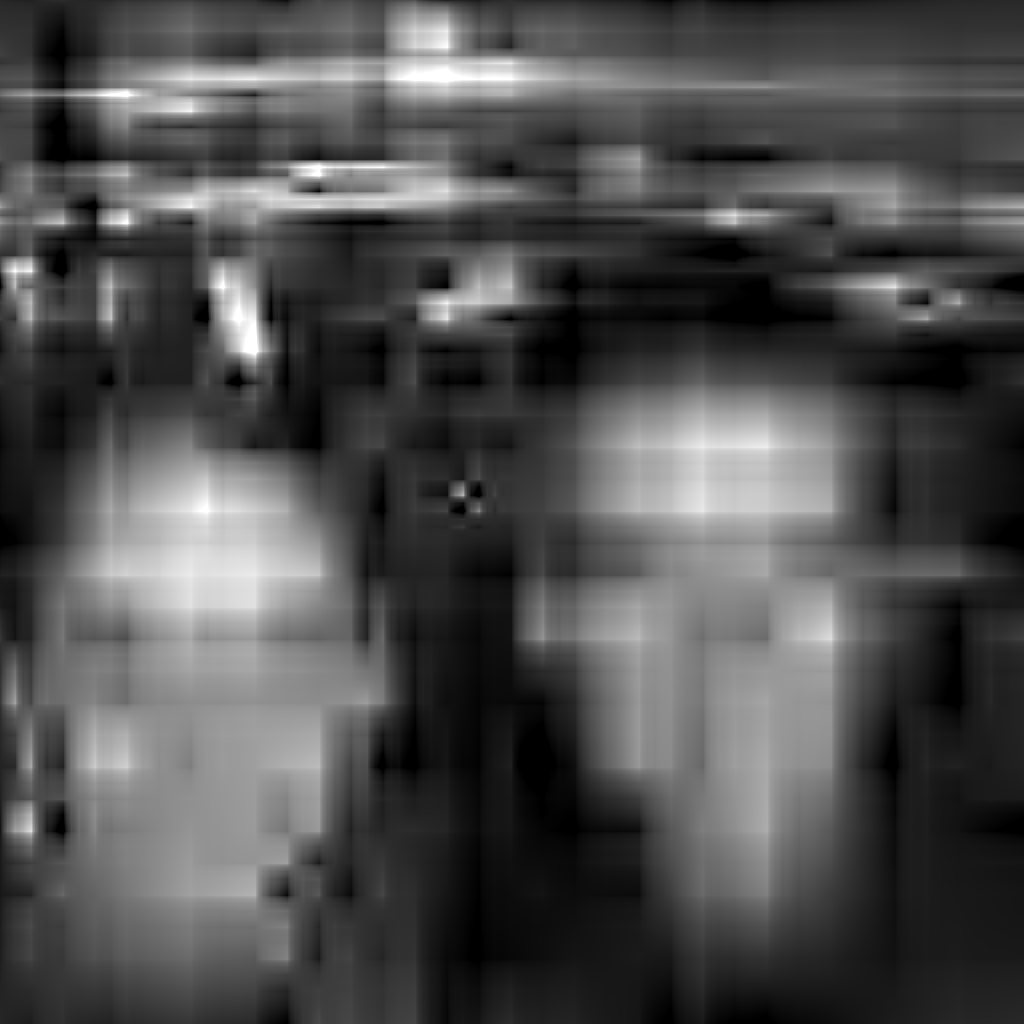
\includegraphics[width=0.3\textwidth]{parijs.png}
	\caption{My girlfriend an I in Paris. Still romantic with only 200 coefficients.}
\end{figure}


\todo{Appendix: some source code}


\nocite{*}
\bibliographystyle{alpha}
\bibliography{references}{}


\end{document}